\chapter{Esercizi Reliability}   

	\section{Esercizio 1}
	Calcolare la reliability di R(t) e l'MTTF del sistema il cui diagramma di reliability è mostrato in figura. Nel calcolare l'MTTF assumere che tutti i componenti siano uguali e che falliscano randomicamente con failure rate pari a $\lambda$.
	
	\begin{figure}[H]
		\centering
		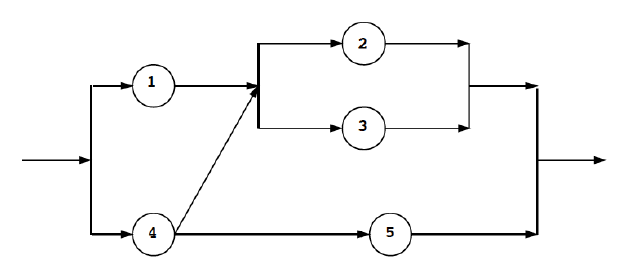
\includegraphics[scale=0.8]{./immagine/reliability_es1.png}
		\caption{Diagramma di reliability del sistema}
		\label{fig:reliability_es1}
	\end{figure}
	
	Tale sistema non è nella forma serie-parallelo, quindi lo riconduciamo ad un sistema del genere scegliendo un componente che viene considerato una volta come funzionante e una volta no, utilizzando poi la seguente relazione che viene dalla regola di Bayes.\\\\
	$R_{sys}=R_{m}P(System\;works|m\;works)+(1-R_{m})P(System\;works|m\;fails) $\\\\
	Il componente scelto è il numero 4, in quanto si ritiene che tale scelta possa semplificare maggiormente il diagramma. Considerando il componente 4 come funzionante, esso viene sostituito con un corto circuito, quindi si elimina anche il componente 1.\\
	A questo punto si può già calcolare la reliability dei due componenti in parallelo 2 e 3:\\\\
	$ R_{23}=1-(1-R_{m})^{2}=1-(1+R_{m}^{2}-2R_{m})=-R^{2}_{m}+2R_{m}=>$\\\\
	$ => 1-R_{23}=(1-R_{m})^{2} $\\\\
	Calcolo la probabilità che il sistema funzioni dato il componente 4 funzionante:\\\\
	$ P(sys\;works|4\;works)=1-(1-R_{m})(1-R_{23})=1-(1-R_{m})^{3}=\\=R_{m}^{3}+3R_{m}-3R_{m}^{2} $\\\\
	Considero ora il componente 4 come non funzionante, quindi viene sostituito con un circuito aperto. Di conseguenza si elimina il componente 5.\\
	Calcolo la probabilità che il sistema funzioni dato il componente 4 non funzionante:\\\\
	$ P(sys\;works|4\;fails)=R_{m}R_{23}=2R_{m}^{2}-R_{m}^{3} $\\\\
	A questo punto posso calcolare la reliability del sistema:\\\\
	$ R_{sys}=R_{m}^{4}+3R_{m}^{2}-3R_{m}^{3}+(1-R_{m})(2R_{m}^{2}-R_{m}^{3})=R_{m}^{4}+3R_{m}^{2}-3R_{m}^{3}+2R_{m}^{2}-\\+R_{m}^{3}-2R_{m}^{3}+R_{m}^{4}=2R_{m}^{4}-6R_{m}^{3}+5R_{m}^{2} $\\\\
	Assumendo che l'andamento della reliability sia un esponenziale negativo, posso così calcolare l'MTTF facendone l'integrale tra 0 e $\infty$.\\\\
	$ MTTF=\int_{0}^{\infty}R_{sys}(t)\;dt=\int_{0}^{\infty}2e^{-4\lambda t}-6e^{-3\lambda t}+5e^{-2\lambda t}\;dt=\\=2*\frac{1}{4\lambda}-6*\frac{1}{3\lambda}+5*\frac{1}{2\lambda}=\frac{1}{\lambda}*(\frac{1}{2}-2+\frac{5}{2})=\frac{1}{\lambda} $\\\\
	In conclusione, quindi, possiamo dire che l'MTTF del sistema complessivo coincide con quello del singolo componente.\\\\
	$ MTTF_{sys}=MTTF_{simplex} $
	
	\section{Esercizio 2}
	Si vogliono mettere a confronto due schemi che cercano di aumentare la reliability di 	un sistema usando ridondanza. Supponiamo che il sistema abbia bisogno di s componenti identici in serie per le proprie operazioni. Supponiamo anche che siano 	dati ($m*s$) componenti. Quale dei due schemi mostrati in figura fornirà una reliability 	maggiore? Considerando che la reliability di un singolo componente sia r, deriva le espressioni per le reliability delle due configurazioni. Confronta le due espressioni per m=3 e s=3.
	
	\begin{figure}[H]
		\centering
		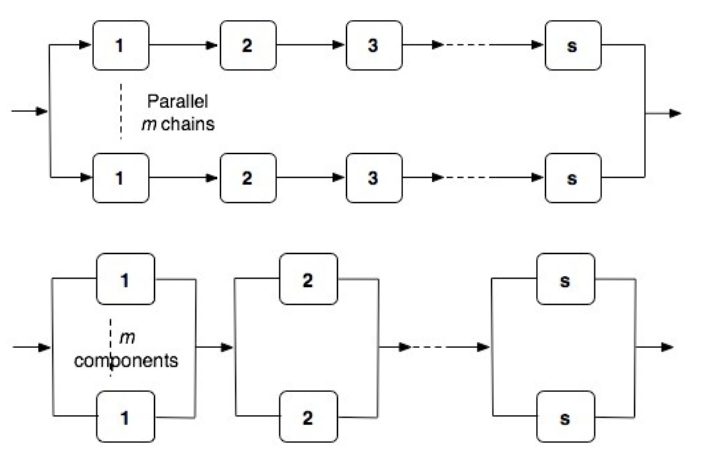
\includegraphics[scale=0.8]{./immagine/reliability_es2.png}
		\caption{Due diversi schemi del sistema che adottano la ridondanza}
		\label{fig:reliability_es2}
	\end{figure}
	
	A occhio si nota subito che il secondo schema è migliore del primo qualunque siano m ed s. Difatti, mentre nel primo caso deve funzionare per forza ogni componente di una delle m serie affinché il sistema funzioni, nel secondo invece per ognuno degli m componenti in parallelo, basta che ne funzioni uno affinché funzioni tutto il sistema. Quindi si può dire che ci sono più probabilità che il primo sistema fallisca.\\
	Riportiamo ora le espressioni delle reliability dei due sistemi:\\\\
	$ R_{sys1}=1-\prod_{i=1}^{m}(1-\prod_{j=1}^{s}r_{ij}) $\\\\
	$ R_{sys2}=\prod_{j=1}^{s}[1-\prod_{i=1}^{m}(1-r_{ij})] $\\\\
	Dato che i componenti sono tutti uguali, essi hanno le stesse reliability quindi posso scrivere le espressioni precedenti come segue:\\\\
	$ R_{sys1}=1-(1-r^{s})^{m} $\\\\
	$ R_{sys2}=(1-(1-r)^{m})^{s} $\\\\
	A questo punto bisogna confrontare le due espressioni per m=3 e s=3.\\\\
	$ R_{sys1}=1-(1-r^{3})^{3} $\\\\
	$ R_{sys2}=(1-(1-r)^{3})^{3} $\\\\
	Considerando la reliability come un esponenziale negativo e fissando un certo failure rate $\lambda$, si confrontano su un grafico le curve della reliability dei due sistemi.
	
	\begin{figure}[H]
		\centering
		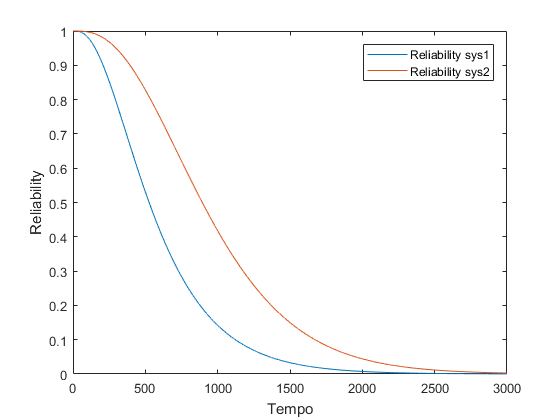
\includegraphics[scale=0.75]{./immagine/grafico_rel_es2.png}
		\caption{Grafico reliability dei sistemi al variare del tempo}
		\label{fig:grafico_rel_es2}
	\end{figure} 
	
	Come si nota dal grafico, la reliability del secondo sistema risulta essere sempre maggiore di quella del primo.
	
	\section{Esercizio 3}
	L'architettura di una rete di computer in un sistema bancario è mostrata in 	figura. L'architettura è chiamata rete a skip-ring ed è progettata per permettere ai processori di comunicare anche dopo che si sono presentati dei fallimenti di alcuni nodi. Ad esempio, se fallisce il nodo 1, il nodo 8 può bypassare il nodo fallito istradando i dati su un link alternativo che va dal nodo 8 al nodo 2. Assumendo che i collegamenti siano perfetti e che ogni nodo abbia una reliability $R_{m}$, deriva un'espressione per la reliability della rete. Se $R_{m}$ obbedisce alla legge di fallimento esponenziale e il failure rate di ogni nodo è 0.005 fallimenti all'ora, determina la reliability del sistema al termine di un periodo di 48 ore.
	
	\begin{figure}[H]
		\centering
		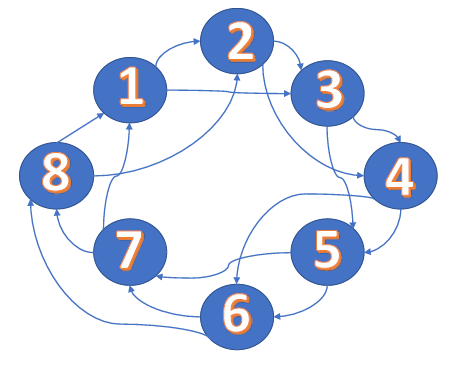
\includegraphics[scale=0.8]{./immagine/reliability_es3.png}
		\caption{Architettura rete di computer}
		\label{fig:reliability_es3}
	\end{figure}
	
	In un certo intervallo di tempo possono fallire da 0 a 8 nodi. Il fallimento del sistema si ha quando falliscono due nodi consecutivi. Quindi la reliability del sistema non è altro che la probabilità che il sistema funzioni in un intervallo di tempo. Tale probabilità si calcola come:\\
	 $ P(sys\;works)=\sum_{k=0}^{8}P(sys\;works|k\;of\;8\;nodes\;work)P(k\;of\;8\;nodes\;work) $\\\\
	 Essendo tutti i nodi indipendenti ed identici con stessa reliability $R_{m}$, la probabilità che k nodi su 8 non falliscano si calcola come il prodotto della probabilità che k nodi non falliscano per la probabilità che 8-k nodi falliscano, il tutto moltiplicato per il numero di configurazioni in cui si verifica questo evento, ottenibile tramite il coefficiente binomiale. Quindi si può scrivere:\\\\
	$ P(k\;of\;8\;nodes\;work)=\binom{8}{k}(R_{m})^{k}(1-R_{m})^{8-k} $\\\\
	Come detto in precedenza il sistema non funziona se ci sono almeno due nodi consecutivi non funzionanti, quindi la probabilità a posteriori dell'espressione precedente si calcola come il rapporto del numero di configurazioni in cui questo non accade (con k nodi funzionanti), fratto il numero di configurazioni in cui ci sono k nodi funzionanti su 8, ovvero il coefficiente binomiale nominato in precedenza.\\
	Tali probabilità sono riportate nella seguente tabella.
	
	\begin{table}[H]
		\footnotesize
		\caption{Probabilità a-posteriori}
		\label{tab:rel_tab}
		\centering
		\begin{tabular}{cc}
			\toprule
			\textbf{Numero nodi funzionanti}&\textbf{P(sys works|k of 8 nodes work)}\\
			\midrule
			0 & 0\\
			\midrule
			1 & 0\\
			\midrule
			2 & 0\\
			\midrule
			3 & 0\\
			\midrule
			4 & $\frac{2}{70}$\\
			\midrule
			5 & $ \frac{16}{56} $\\
			\midrule
			6 & $\frac{20}{28} $\\
			\midrule
			7 & 1\\
			\midrule
			8 & 1\\
			\bottomrule
			
		\end{tabular}
	\end{table} 
	 
	 La reliability del sistema sarà quindi:\\\\
	 $ R_{sys}=\sum_{k=0}^{8}P(sys\;works|k\;of\;8\;nodes\;work)*\binom{8}{k}(R_{m})^{k}(1-R_{m})^{8-k}=\\\\
	 =\frac{2}{70}*70*(R_{m}^{4})(1-R_{m})^{4}+\frac{16}{56}*56*(R_{m}^{5})(1-R_{m})^{3}+\frac{20}{28}*28*(R_{m}^{6})(1-R_{m})^{2}+8*(R_{m}^{7})(1-R_{m})+R_{m}^{8} $\\\\
	 Valutiamo ora la reliability dopo un periodo di 48 ore, supponendo abbia una distribuzione esponenziale e il failure rate sia 0.005.
	
	\begin{figure}[H]
		\centering
		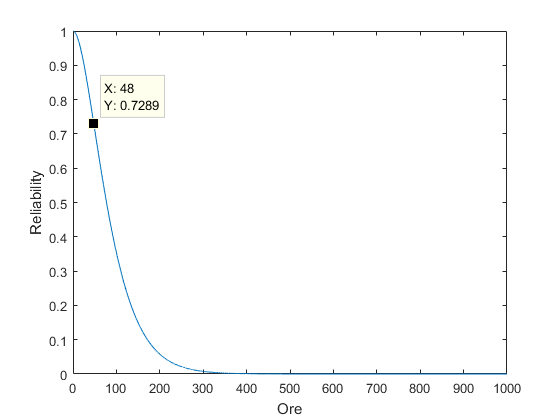
\includegraphics[scale=0.75]{./immagine/grafico_rel_es3.png}
		\caption{Grafico reliability del sistema al variare del tempo con $\lambda=0.005$ }
		\label{fig:grafico_rel_es3}
	\end{figure} 
	
	Come si nota dal grafico, dopo 48 ore la reliability è 0.7289.\\\\
	
	\section{Esercizio 4}
	Un'applicazione richiede che almeno 3 processori di un sistema multiprocessore siano disponibili con più del 99\% di probabilità. Il costo di un processore con l’80\% di reliability è 1000\$ e ogni incremento del 10\% in reliability costa 500\$. Determinare il numero di processori (n) e la reliability (p) di ogni processore (assumere che tutti i processori abbiano la stessa reliability) che minimizzi il costo totale del sistema.\\\\
	Dato che si richiede debbano funzionare 3 processori su 3, questo sistema può essere visto come un 3-out-of-N system, la cui reliability sarà:\\\\
	$ R_{sys}=\sum_{i=0}^{N-3}\binom{N}{i}R_{m}^{N-i}(1-R_{m})^{i} $ \\\\
	Ora bisogna trovare il numero di processori N che minimizzi il costo e garantisca una reliability di almeno 2 nines.\\
	Per i singoli processori è possibile avere solo 3 valori di reliability incrementandola ogni volta del 10\%, ovvero 0.8, 0.88 e 0.96, questo perché non posso avere un valore di reliability superiore a 1.\\
	Usando l'espressione precedente, tramite Matlab, sono stati calcolati i valori di reliability per diverso numero di processori (enumerazione), fino a che non si è raggiunta una reliability di almeno 0.99.\\
	Vediamo i risultati ottenuti, partendo ovviamente da un numero di processori pari a 3.
	
	\begin{table}[H]
		\footnotesize
		\caption{Valori reliability sys al variare di N e della reliability dei processori}
		\label{tab:rel_tab_es4}
		\centering
		\begin{tabular}{cccc}
			\toprule
			\textbf{N} & \textbf{Rm=0.8} & \textbf{Rm=0.88} & \textbf{Rm=0.96}\\
			\midrule
			3 & 0.512 & 0.6815 & 0.8847\\
			\midrule
			4 & 0.8192 & 0.9268 & 0.9909\\
			\midrule
			5 & 0.9421 & 0.9857 & \\
			\midrule
			6 & 0.983 & 0.9975 & \\
			\midrule
			7 & 0.9953 &  & \\
			\bottomrule
			
		\end{tabular}
		
	\end{table}
	Come si nota, con processori aventi 0.8 di reliability, ne sono necessari 7 afinché il sistema abbia una reliability di 2 nines; nel caso di reliability del singolo processore pari a 0.88 ne servono 6 e infine nel caso di reliability pari a 0.96, ne servono solo 2.\\
	Calcoliamo ora i costi in tutti e 3 i casi:\\\\
	$ Costo_{N=7,Rm=0.8}=1000*7=7000\$ $\\\\
	$ Costo_{N=6,Rm=0.88}=1000*6+500*6=9000\$ $\\\\
	$ Costo_{N=2,Rm=0.96}=1000*2+500*2+500*2=4000\$ $\\\\\\
	In conclusione, per minimizzare il costo totale del sistema ed ottenere una reliability di 2 nines, abbiamo bisogno di 2 processori su cui si applicano due aumenti di reliability del 10\%.\\\\\\\\\\
	
	\section{Esercizio 5}
	Il sistema descritto nella figura sottostante è un sistema di elaborazione per un elicottero. Il sistema ha processori dual-ridondanti e unità di interfaccia dual-ridondanti. Sono usati due bus nel sistema e entrambi sono dual-ridondanti. La parte interessante del sistema è l'equipaggiamento di navigazione. Il velivolo può essere completamente navigato usando l'Inertial Navigation System (INS). Se l'INS fallisce, il velivolo può essere navigato usando la combinazione del Doppler e dell'Altitude Heading and Reference System (AHRS). Il sistema contiene tre unità AHRS, di cui solo una è necessaria. Questo è un esempio di ridondanza funzionale dove i dati dall'AHRS e dal Doppler possono essere usati per rimpiazzare l'INS, se esso fallisce. A causa di altri sensori e strumenti, entrambi i bus sono necessari affinché il sistema funzioni correttamente indipendentemente dalla modalità di navigazione per cui esso è impiegato.
	
	\begin{figure}[H]
		\centering
		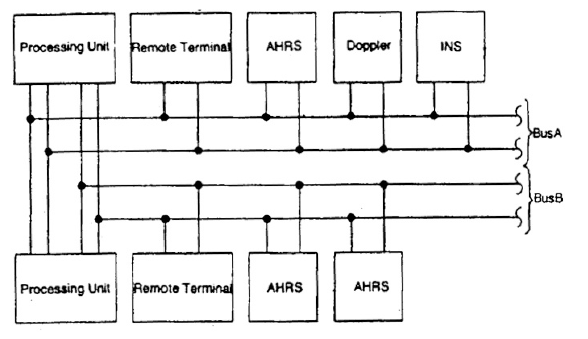
\includegraphics[scale=0.8]{./immagine/reliability_es5.png}
		\caption{Sistema di elaborazione di un elicottero}
		\label{fig:reliability_es5}
	\end{figure}
	
	Di seguito è mostrato il Reliability Block Diagram (RBD) del sistema:
	
	\begin{figure}[H]
		\centering
		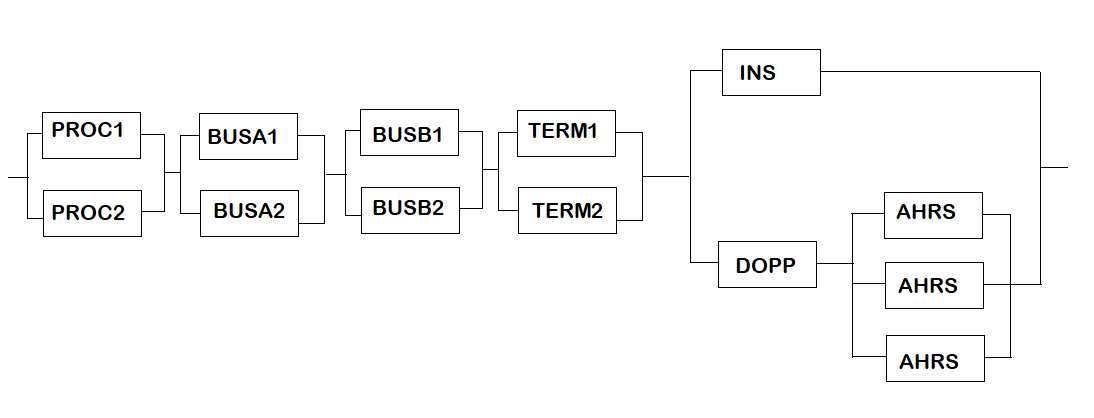
\includegraphics[scale=0.45]{./immagine/rbd_es5.png}
		\caption{Reliability Block Diagram}
		\label{fig:rbd_es5}
	\end{figure}
	
	Di seguito è mostrato il Fault Tree del sistema:
	
	\begin{figure}[H]
		\centering
		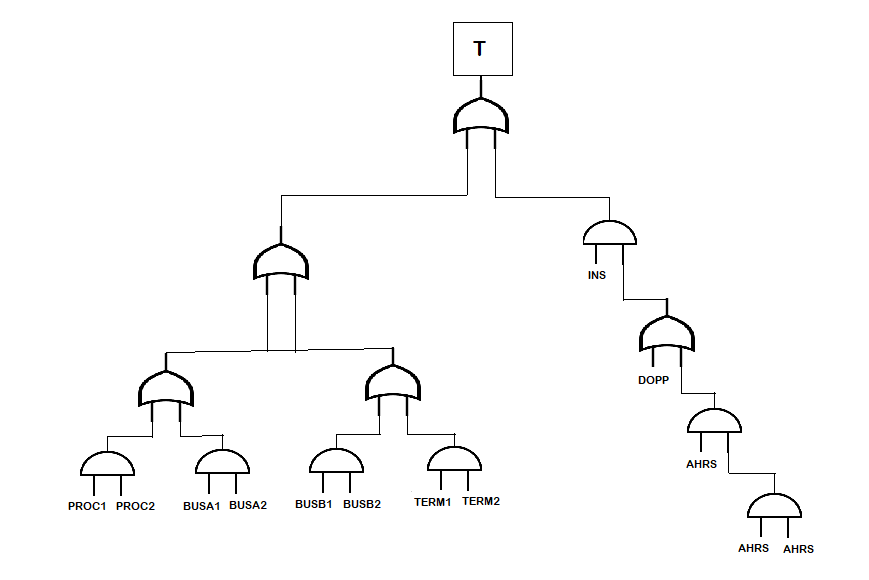
\includegraphics[scale=0.7]{./immagine/fault_tree_es5.png}
		\caption{Fault Tree}
		\label{fig:fault_tree_es5}
	\end{figure}
	
	I minimal cut set saranno:\\\\
	$ M_{1}=(PROC1*PROC2)$\\
	$M_{2}=(BUSA1*BUSA2)$\\$M_{3}=(BUSB1*BUSB2)$\\$M_{4}=(TERM1*TERM2)$\\$M_{5}=(((AHRS*AHRS*AHRS)+DOPP)*INS) $\\\\
	Calcoliamo ora la reliability del sistema per un volo di un'ora tramite le formule per le serie e i paralleli:\\\\
	$ R_{ser}=\prod_{i}^{}R_{i}(t) $\\
	$ R_{par}=1-\prod_{i}^{}(1-R_{i}(t)) $\\\\
	$ R_{sys}=(1-(1-R_{PROC})^{2})*(1-(1-R_{BUS})^{2})^{2}*(1-(1-R_{TERM})^{2})*(1-(1-R_{INS}))*(R_{DOPP}*(1-(1-R_{AHRS})^{3})) $\\\\
	
	Considerando la reliability come un'esponenziale negativo del tipo $ e^{-\lambda t} $ e avendo a disposizione i seguenti valori di MTTF per ogni componente, è possibile calcolare il failure rate di ciascuno e quindi la reliability del sistema ($\lambda=\frac{1}{MTTF}$). Per farlo utilizziamo Matlab.
	
		\begin{figure}[H]
			\centering
			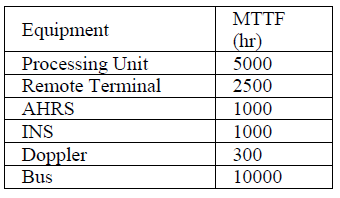
\includegraphics[scale=0.7]{./immagine/mttf_es5.png}
			\caption{MTTF}
			\label{fig:mttf_es5}
		\end{figure}
		
	Otteniamo i seguenti valori di $\lambda$ per ogni componente mostrati in ordine come nella tabella precedente:
	
	\begin{figure}[H]
		\centering
		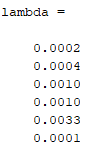
\includegraphics[scale=0.9]{./immagine/lambda_es5.png}
		\caption{Failure Rate}
		\label{fig:lambda_es5}
	\end{figure}
	
	Otteniamo così un valore di reliability pari a 0.9957, quindi di due nines.\\\\
	Ripetiamo ora lo stesso procedimento, includendo però un fattore di coverage c per la fault detection e la riconfigurazione delle processing unit, mantenendo, però, una reliability pari a 0.999999.\\
	La nuova formula da considerare per i processori, che include il fattore di coverage è:\\\\
	$ R_{c}=R_{1}+c*(1-R_{1})*R_{2} $\\\\
	c è la probabilità che, quando un fallimento si presenta, esso è rilevato correttamente. $R_{1}$ e $R_{2}$ sono entrambe uguali a $R_{PROC}$.\\
	Basta quindi calcolare $R_{c}$ in funzione della reliability del sistema, fissata a 0.999999. Si calcola, poi, c (tramite un apposito script Matlab), come:\\\\
	$ c=22.7163$
	
	Non esiste, dunque, un valore di coverage tale da constentire il raggiungimento di una reliability di 6 nines.